\section{Metodology and Results}

% \subsection*{3.1 Setup and Routine Algorithm Optimization}

%     About the python algorithm to turn the experiment autonomous it was made a study and modelling of the software architecture to optimize it 
%     for further control loop application to be implemented.
%     From the changes made until now it highlights:

%     - Integrate high speed camera to the experiment routine.

%     - Remodel the software to support threads in order to separate the sensoring and controlling routines.

%     - Reduce the data collected size. 

%     - Synchronize the power supply step commands and voltage sensoring. 

%     - Reestructure the setup file in order to make it more intuitive to use the experiment. 

%     - Improvements in code organization and readability.

%     About the setup,integrate was changed the liquid, nozzle diameter and distance to the plate in order to make the experiment 
%     the most stable and easy to reach cone-jet mode as possible.
%     For example, while doing experiments we discovered that the frequency of the pump machine internal motors was
%     creating an interference in the flowrate. Therefore compromising the stabilization in cone jet mode.
%     A solution for that was to increase the flowrate wich smooths this pumping noise. For that was also necessary
%     to increase the nozzle diameter to balance with all other variables from the experiment.


% \subsection*{3.2 Experiment 1}

%     This first experiment was made using the setup:

%     - liquid: water60alcohol40

%     - flow rate min: 1.45 mL/hr

%     - config: nozzle to plate

%     - nozzle to plate or ring distance: 1.5 cm

%     - nozzle diameter: 0.136 mm

%     In Figure 5 we can see 5 graphs: 

%     1 - current values measured by the oscilloscope. As it is a lot of data it is compressed in the figure.

%     2 - Voltage step sequence in order to evaluate the dynamics in each high voltage level.

%     3,4,5 - Statistical values measured by each window of 0.5s of data collected. This values will be used in the classification algorithm.
%     Those values are already classified by colour and the legend is showed below.

%     LEGEND:

%     - Green = Dripping

%     - Blue =  Intermittend

%     - Red = Cone Jet mode

%     - Purple = Streamer Onset (high current values)

%     - Black = Undefined

%     \begin{figure}[H]
%         \center
%         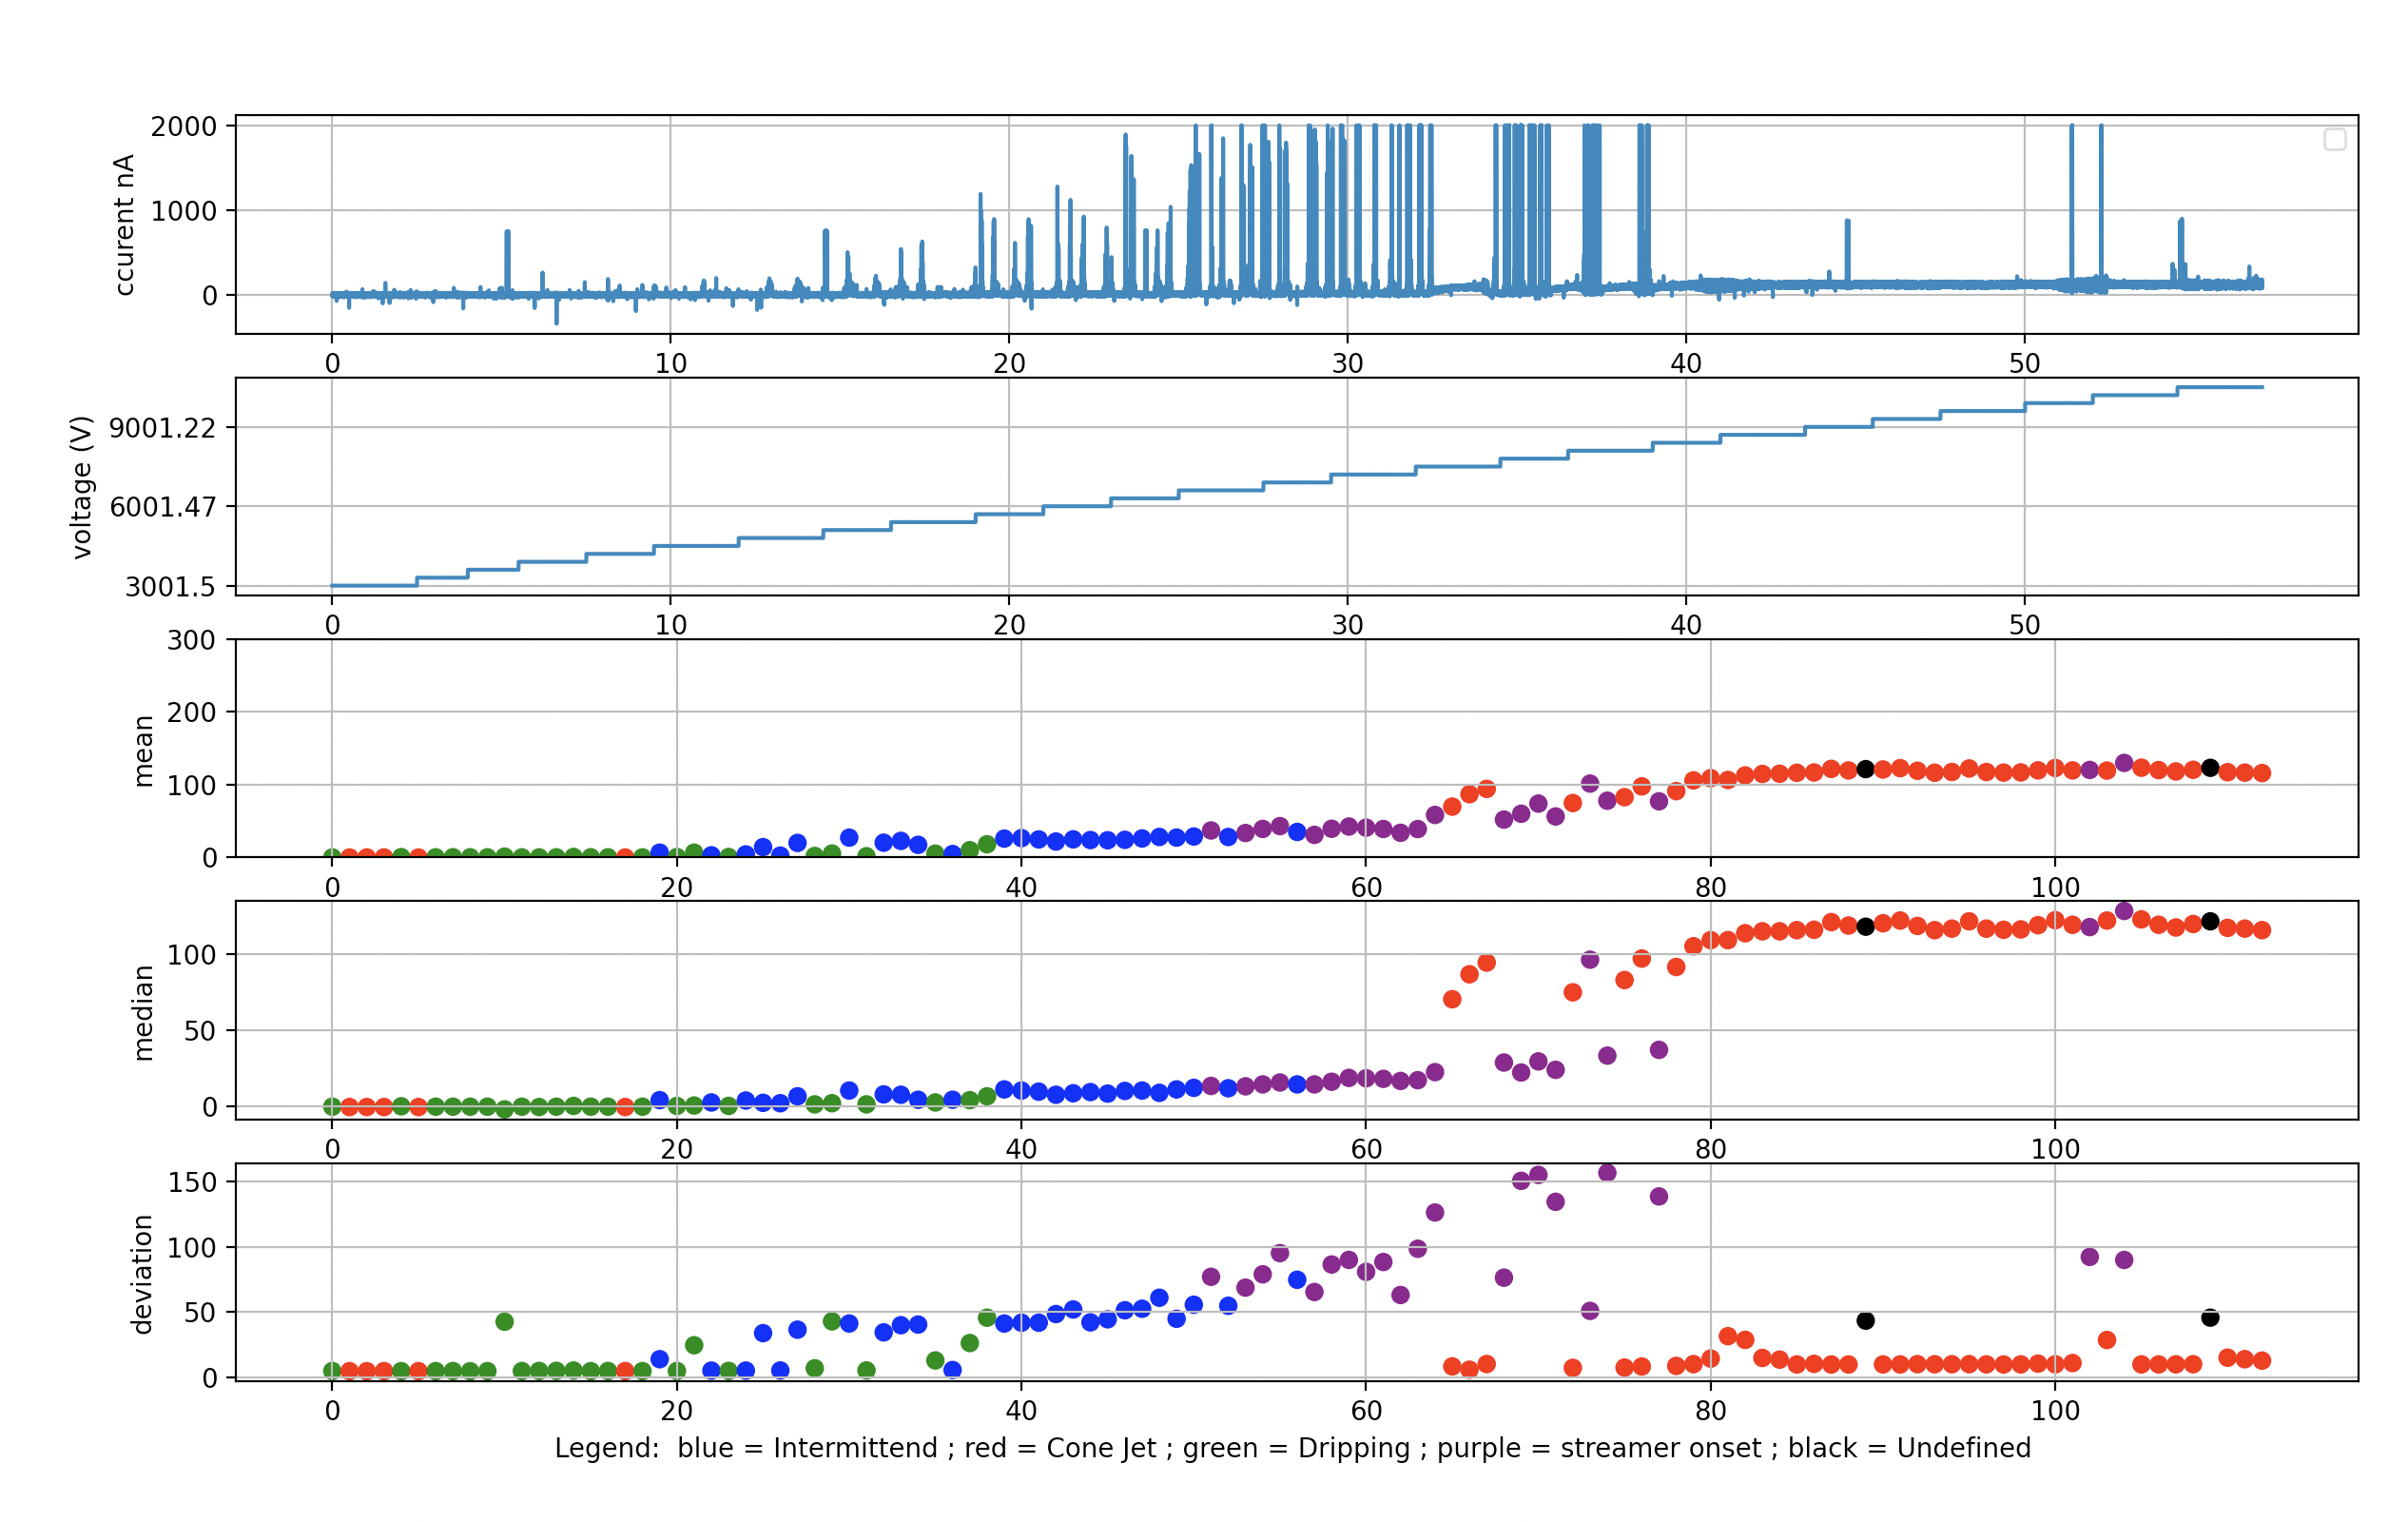
\includegraphics[width=17cm]{images/images_folder_2/img1.png}
%         \caption{Data acquired in the experiment 1 - liquid: Water AND alcohol}
%     \end{figure}

%     In Figure 6 and 7 we can see one data window sample of dripping and one of cone jet dynamics. There are two graphs. The first one its
%     the current datapoints filtered by a ideal low pass butterworth filter. In the second graph we can see the module of the fast fourier transform real values.

%     We can see in Figure 6 that there were two droplets expelled by the nozzle. This can be seen as the two signal waves in the current value and the amount of frequencies seen in the second graph.

%     \begin{figure}[H]
%         \center
%         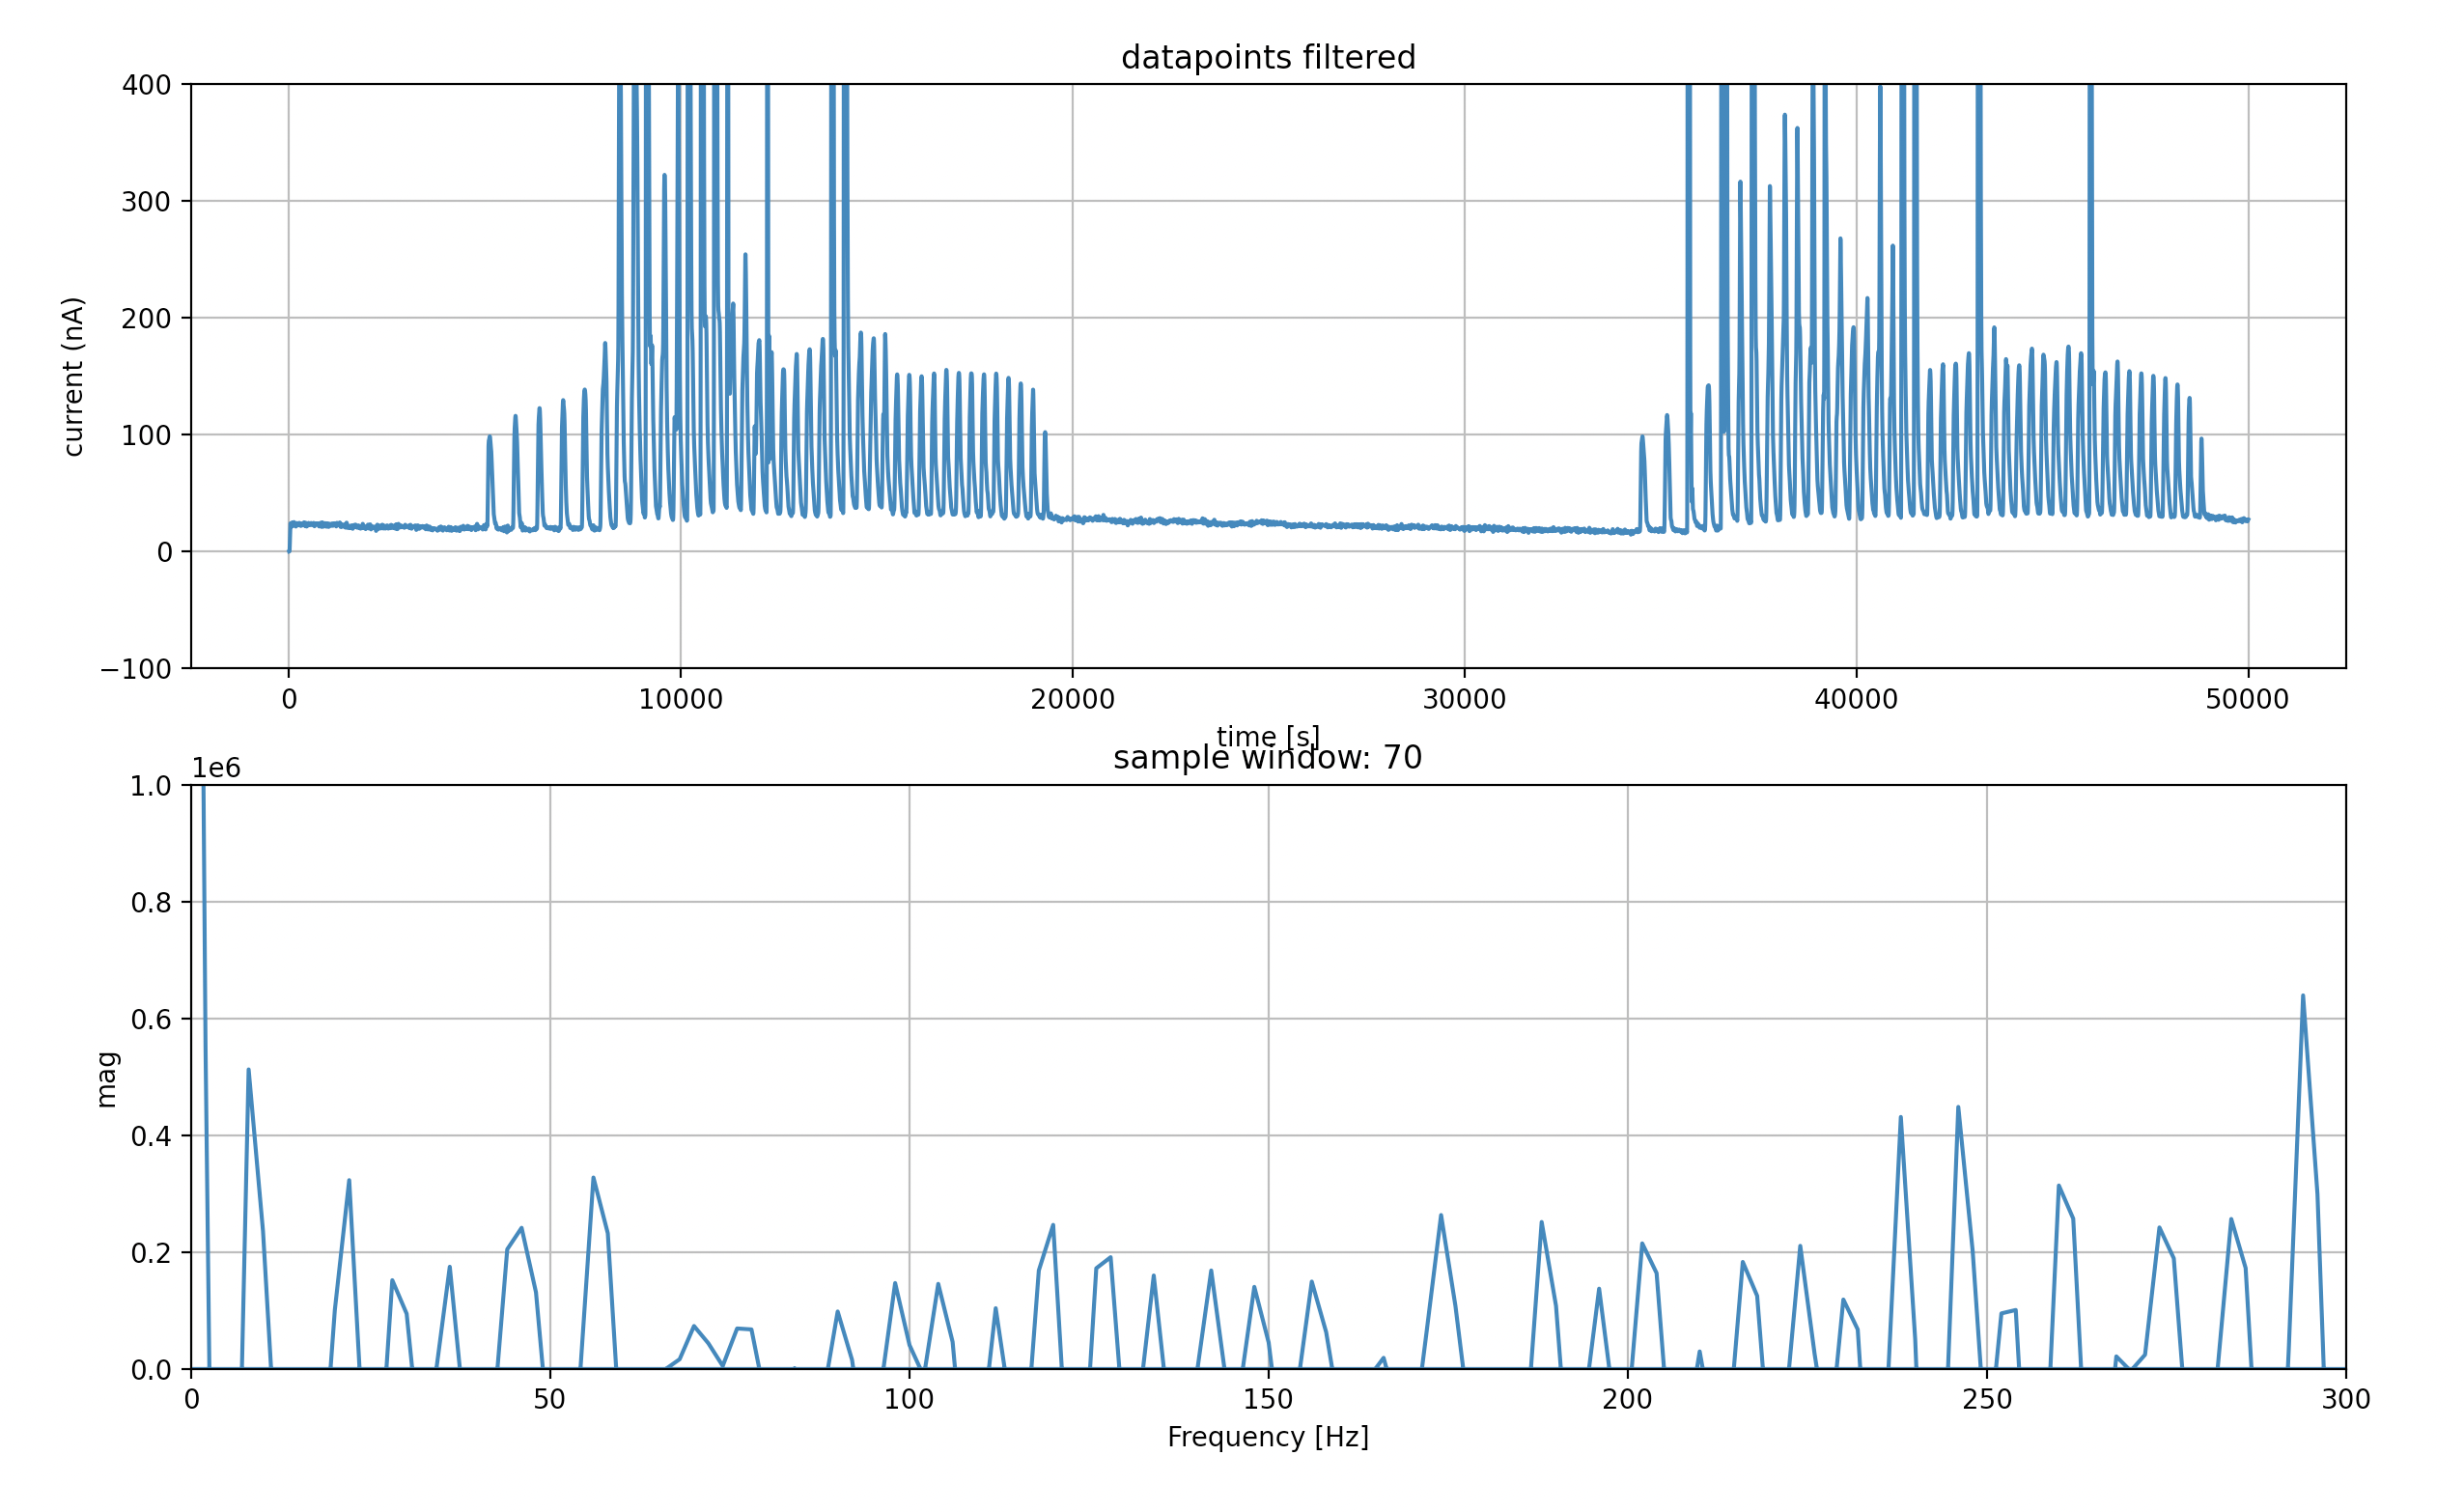
\includegraphics[width=12cm]{images/images_folder_2/img2.png}
%         \caption{Dripping sample}
%     \end{figure}

%     We can see in Figure 7 that the current signal is more stable and also with an offset current arround 100nA showing that the spray is in cone jet mode. Also seen as the 0 Hz DC component value in the frequency domain graph.


%     \begin{figure}[H]
%         \center
%         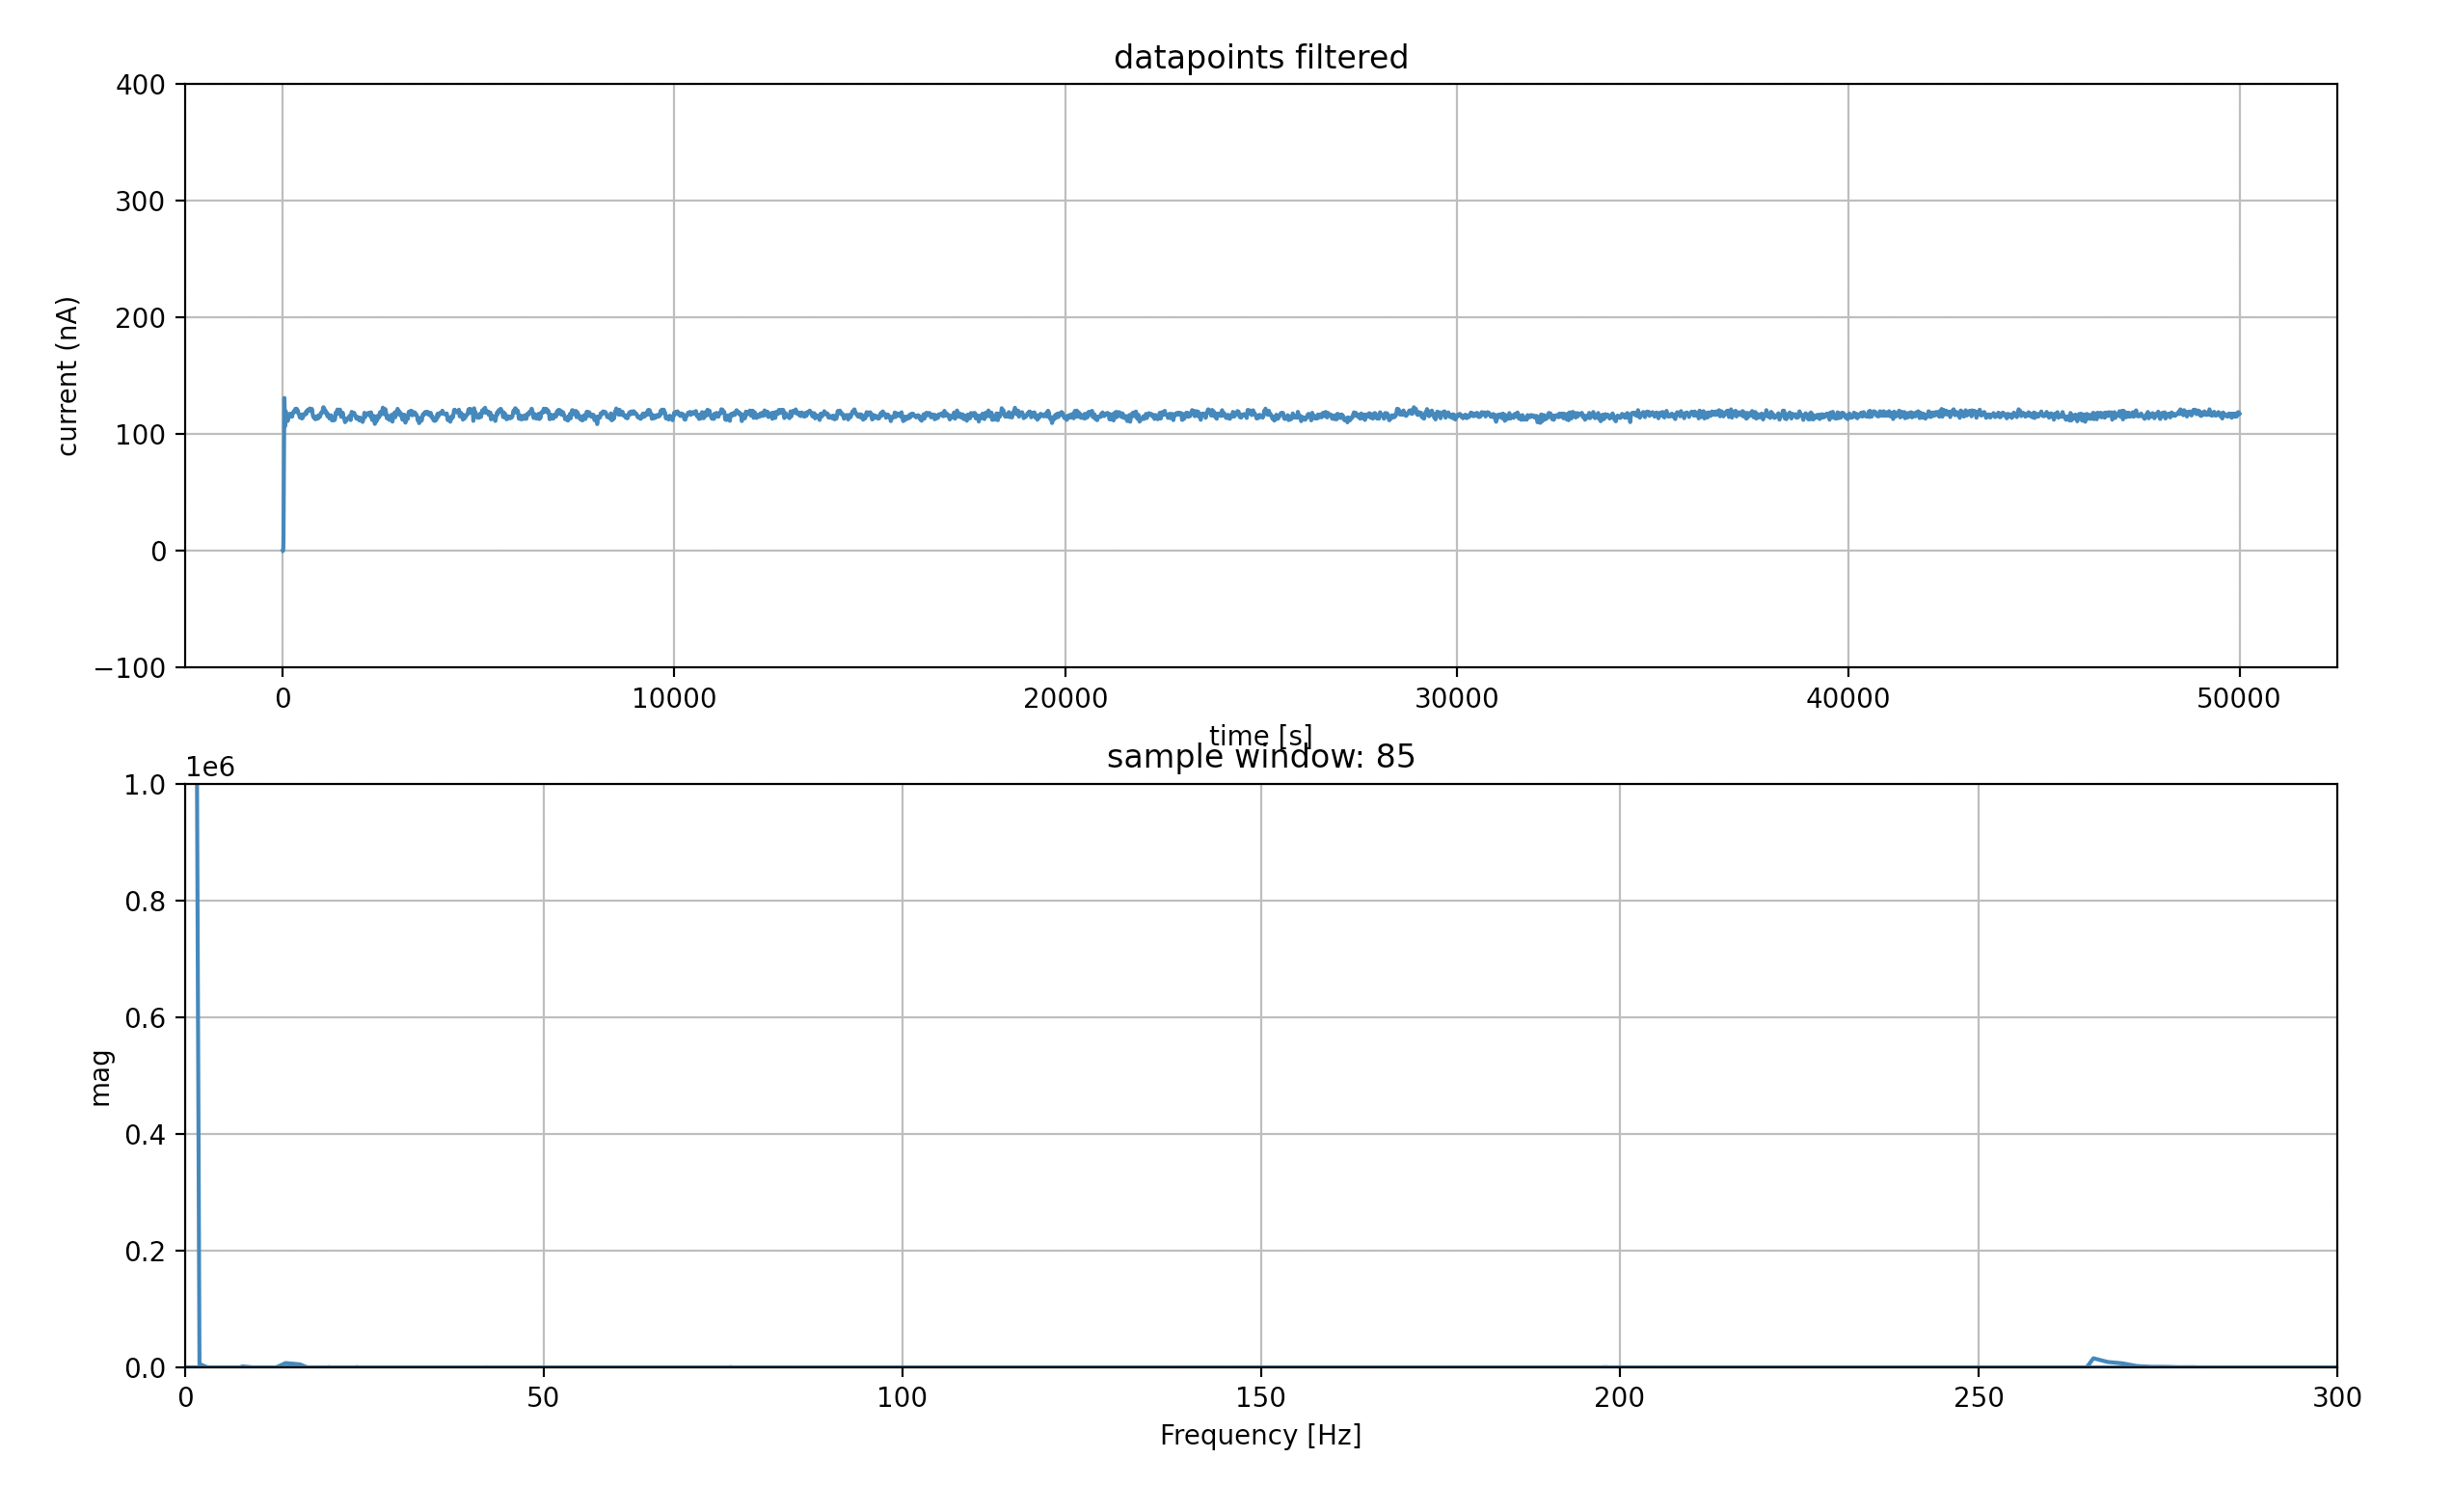
\includegraphics[width=12cm]{images/images_folder_2/img3.png}
%         \caption{Cone jet sample}
%     \end{figure}

%     Other interesting grahps exposed in Sjaaks\cite*[]{Sjaaks} paper is correlating statistical values relations to each voltage step and classification. This is also good to evaluate the separability of each classification method.
%     Those graphs can be seen in Figures 8, 9 and 10.

%     \begin{multicols}{3}

%         \begin{figure}[H]
%             \center
%             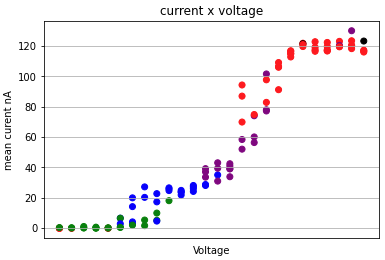
\includegraphics[width=5cm]{images/images_folder_3/data2_sjaaksgraph1.png}
%             \caption{mean current X voltage}
%         \end{figure}


%         \begin{figure}[H]
%             \center
%             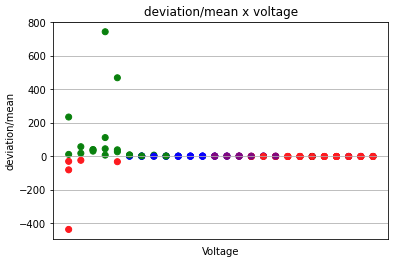
\includegraphics[width=5cm]{images/images_folder_3/data2_sjaaksgraph2.png}
%             \caption{deviation/mean}
%         \end{figure}


%         \begin{figure}[H]
%             \center
%             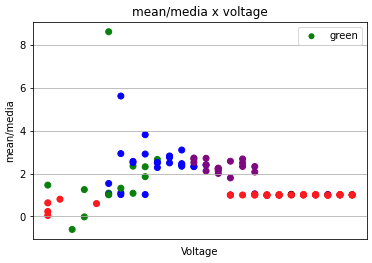
\includegraphics[width=5cm]{images/images_folder_3/data2_sjaaksgraph3.png}
%             \caption{mean/median}
%         \end{figure}

%     \end{multicols}



% \subsection*{3.3 Experiment 2}

% In this experiment the liquid was changed in order to have a bigger voltage range in the cone jet mode. Which is the most valuable mode in this project.

%     - liquid: ethanol pure
    
%     - flow rate min: 1.5 mL/hr
    
%     - camera to nozzle distance: 16.5 cm
    
%     - config: nozzle to plate
    
%     - nozzle to plate or ring distance: 1.5 cm
    
%     - nozzle diameter: 0.136 mm

%     - type of measurement: 

%         * voltage start: 3000 V

%         * voltage stop: 10000 V

%         * step size: 100 V 

%         * step time: 5 s

%     In Figure 11, the data is well classified but it also have a noise in the system that can been seen in the peak current values.
%     Those peaks can be seen in all the voltage ranges in this experiment and also have similar distances in beetween the peaks. This is probably caused by
%     external interference but it is still not certain what is it about.

%     \begin{figure}[H]
%         \center
%         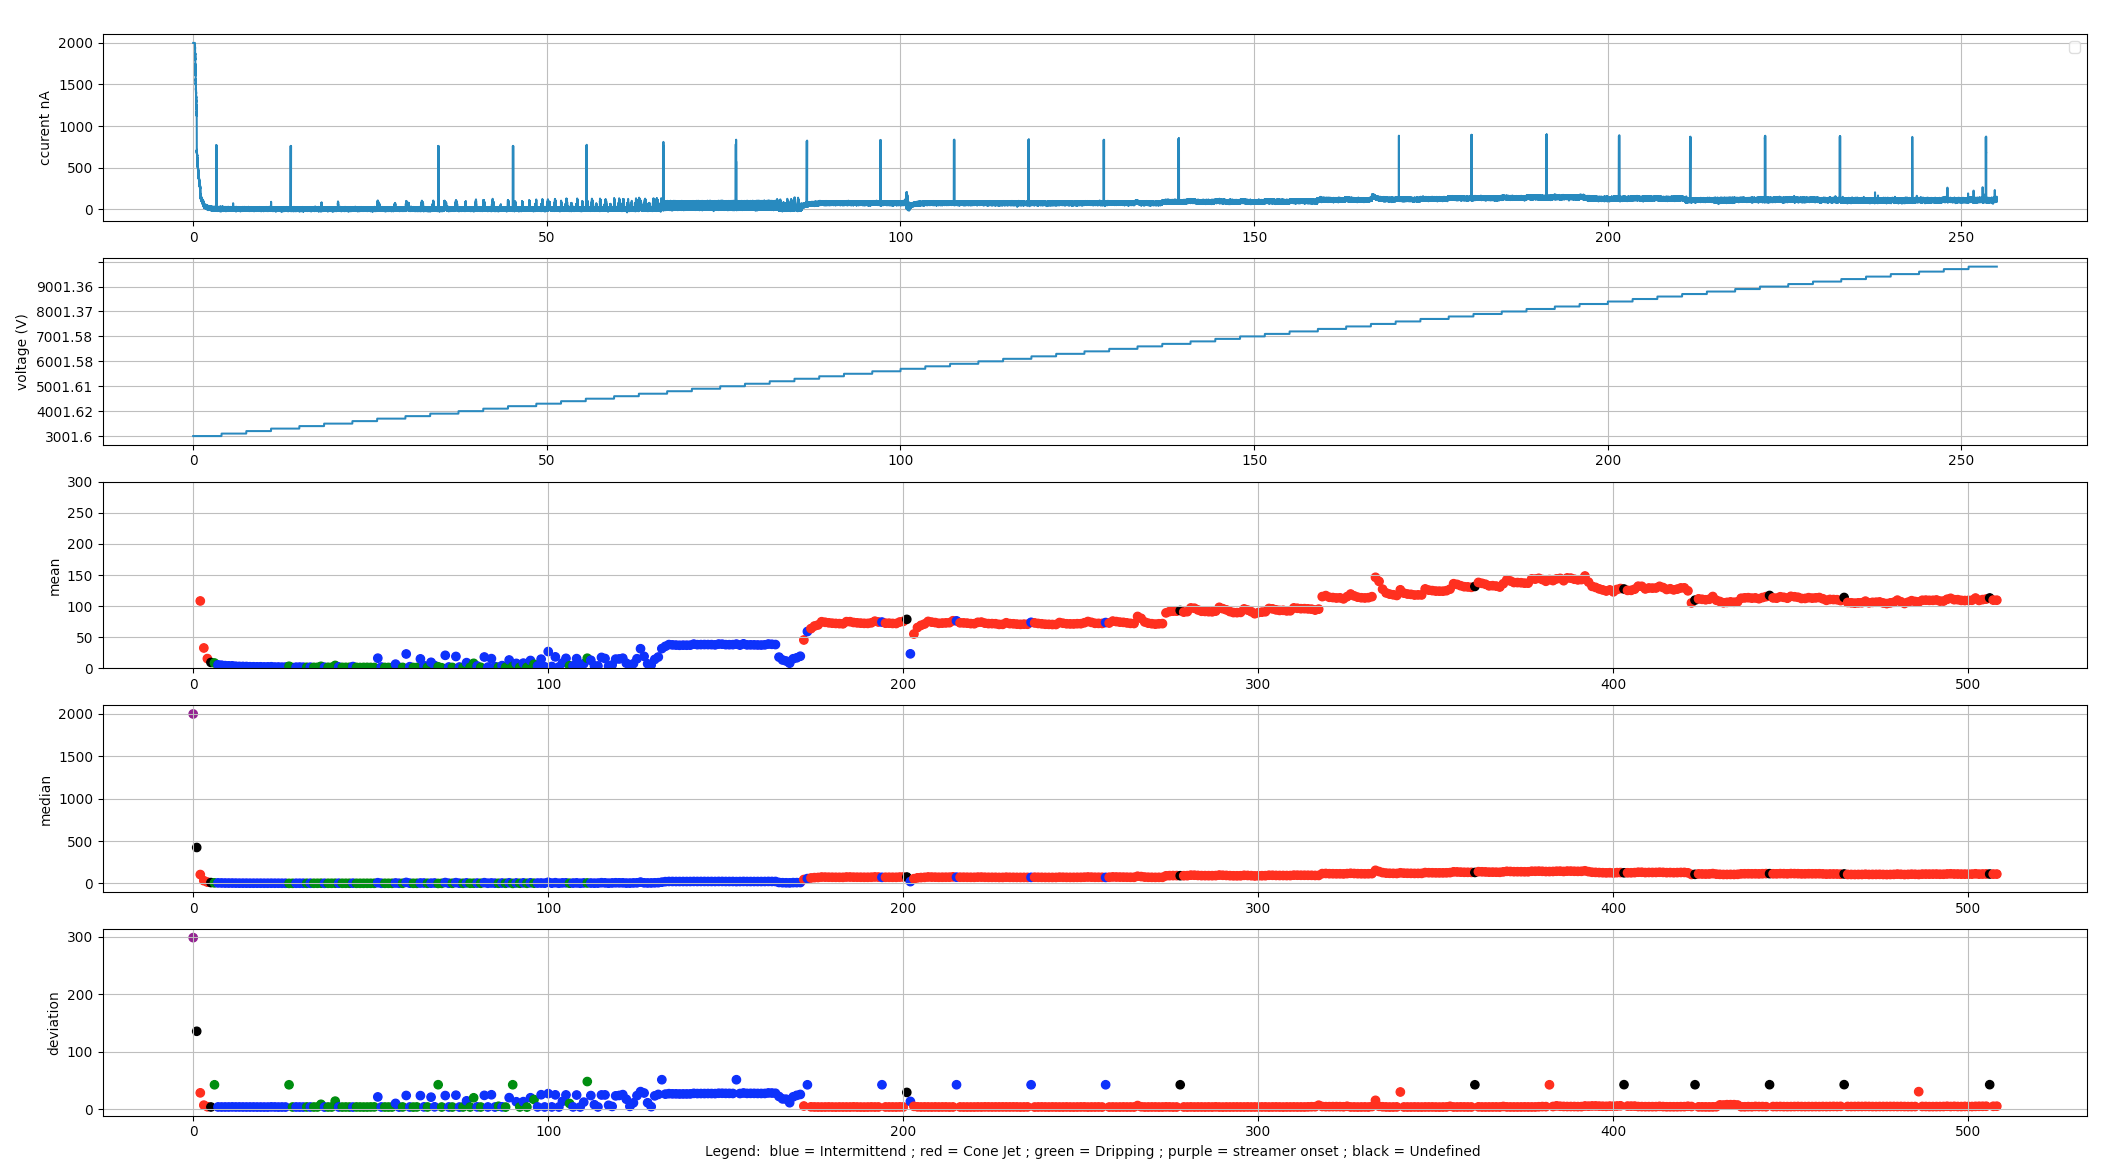
\includegraphics[width=17cm]{images/images_folder_3/data3.png}
%         \caption{Data acquired in the experiment 2 - pure ethanol}
%     \end{figure}

%     The Figure 12 shows the same current x time graph but with a zoom in y axis in order to see the signal steps in the experiment. It is also classified by the same color legend as all graphs in this overview.



%     \begin{figure}[H]
%         \center
%         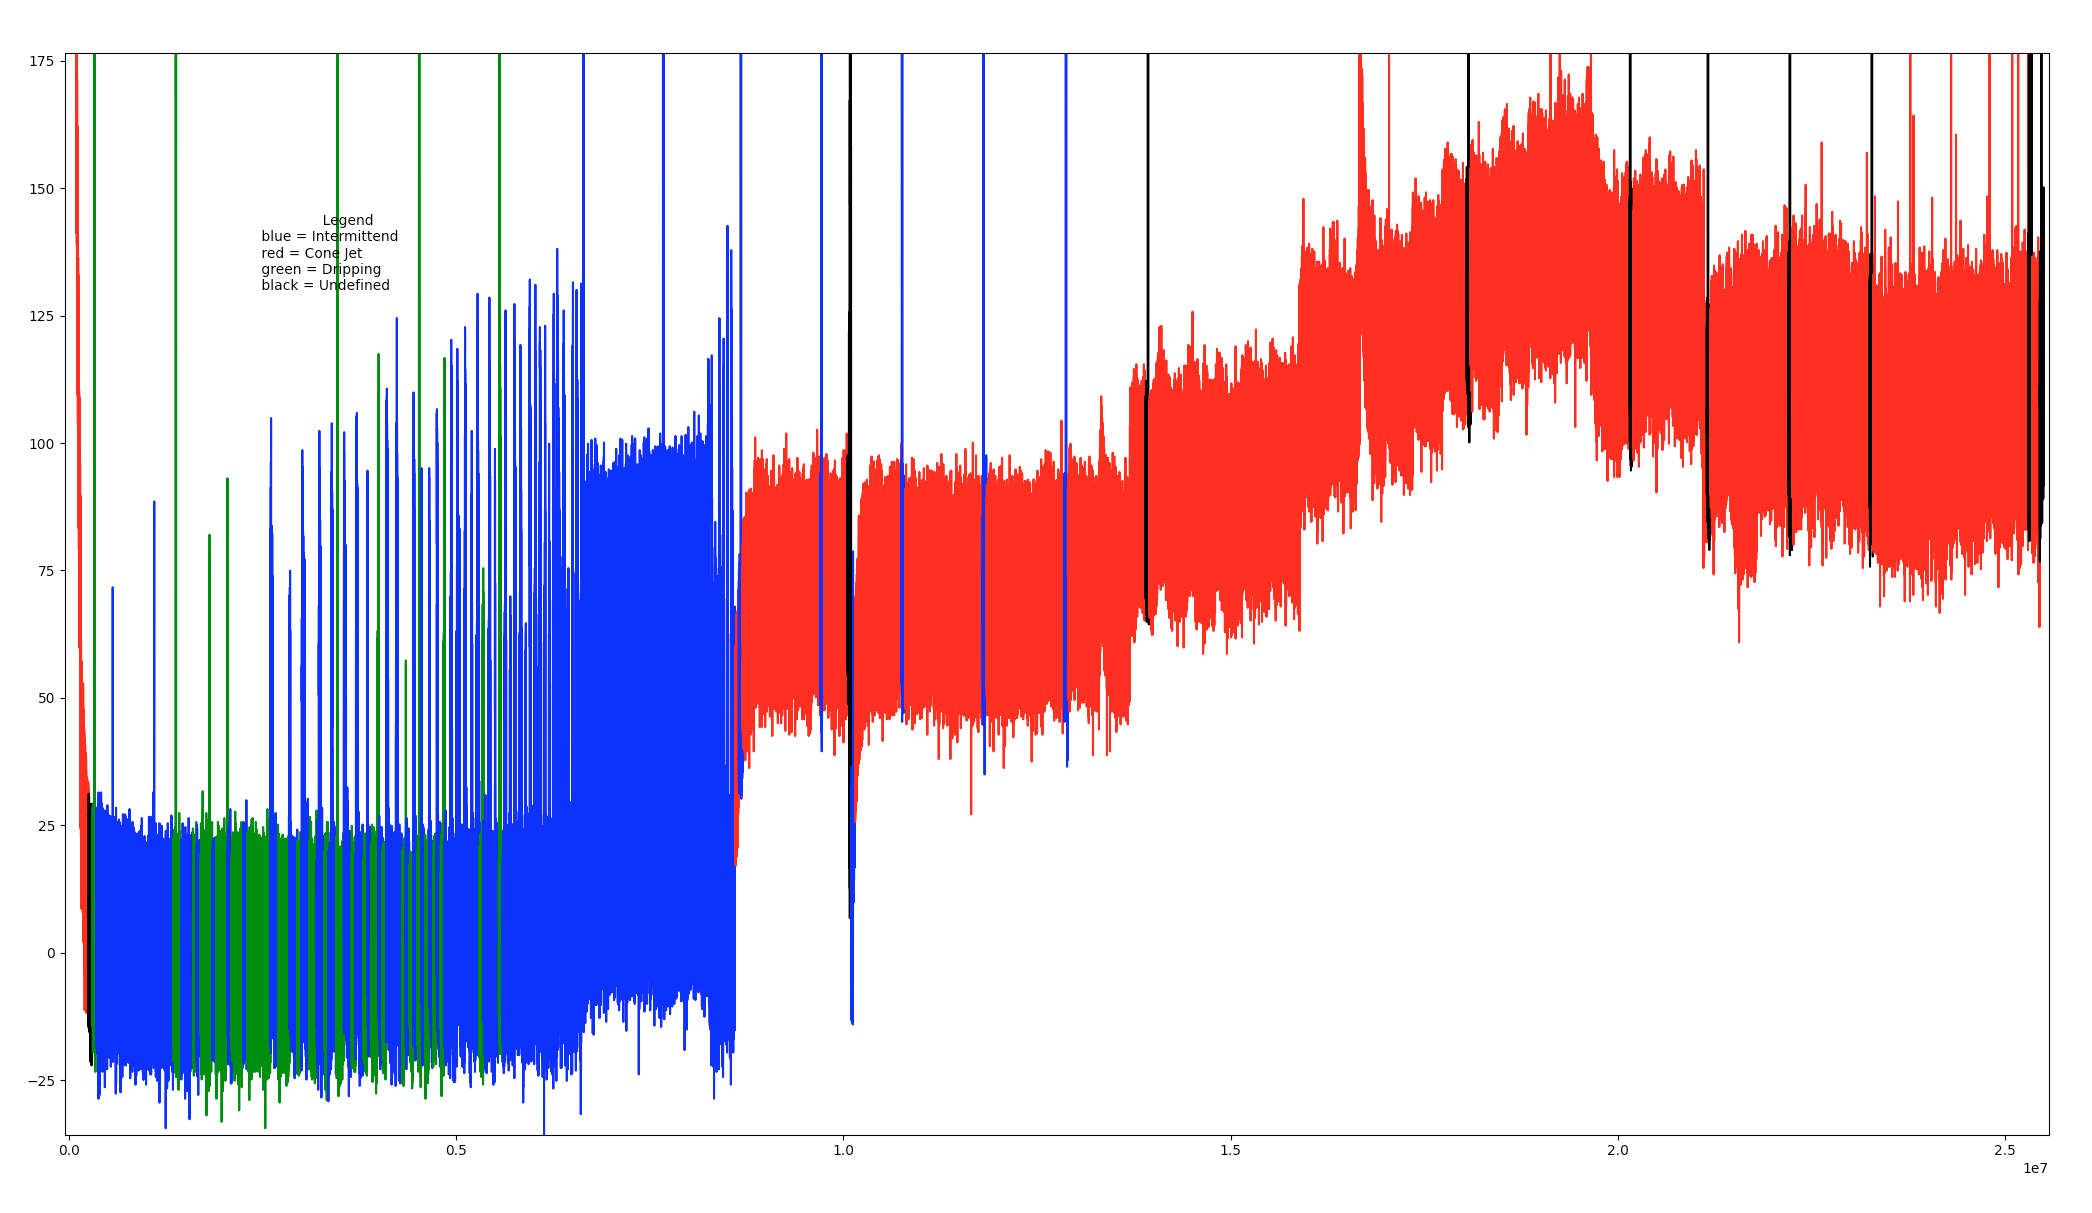
\includegraphics[width=15cm]{images/images_folder_3/data3current.png}
%         \caption{current graph with classification}
%     \end{figure}

%     The Figures 13, 14 and 15 shows graphs with statistical realations in the data. 


%     \begin{multicols}{3}

%         \begin{figure}[H]
%             \center
%             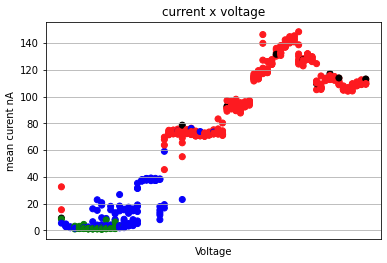
\includegraphics[width=5cm]{images/images_folder_3/data3_sjaaksgraph1.png}
%             \caption{current mean X voltage}
%         \end{figure}

%         \begin{figure}[H]
%             \center
%             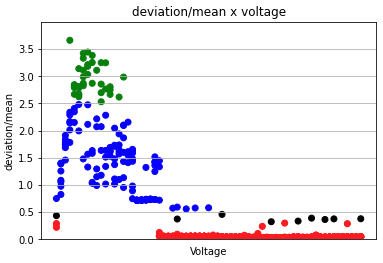
\includegraphics[width=5cm]{images/images_folder_3/data3_sjaaksgraph2.png}
%             \caption{deviation/mean}
%         \end{figure}

%         \begin{figure}[H]
%             \center
%             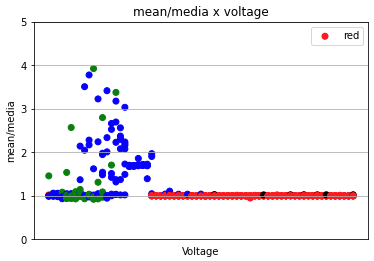
\includegraphics[width=5cm]{images/images_folder_3/data3_sjaaksgraph3.png}
%             \caption{mean/median}
%         \end{figure}

%     \end{multicols}


% \subsection*{3.4 Experiment 3}

%     - liquid: ethanol pure
        
%     - flow rate min: 1.5 mL/hr

%     - camera to nozzle distance: 16.5 cm

%     - config: nozzle to plate

%     - nozzle to plate or ring distance: 1.5 cm

%     - nozzle diameter: 0.136 mm

%     - type of measurement: 

%         * voltage start: 3000 V

%         * voltage stop: 11000 V

%         * step size: 50 V 

%         * step time: 1 s

%     \begin{figure}[H]
%         \center
%         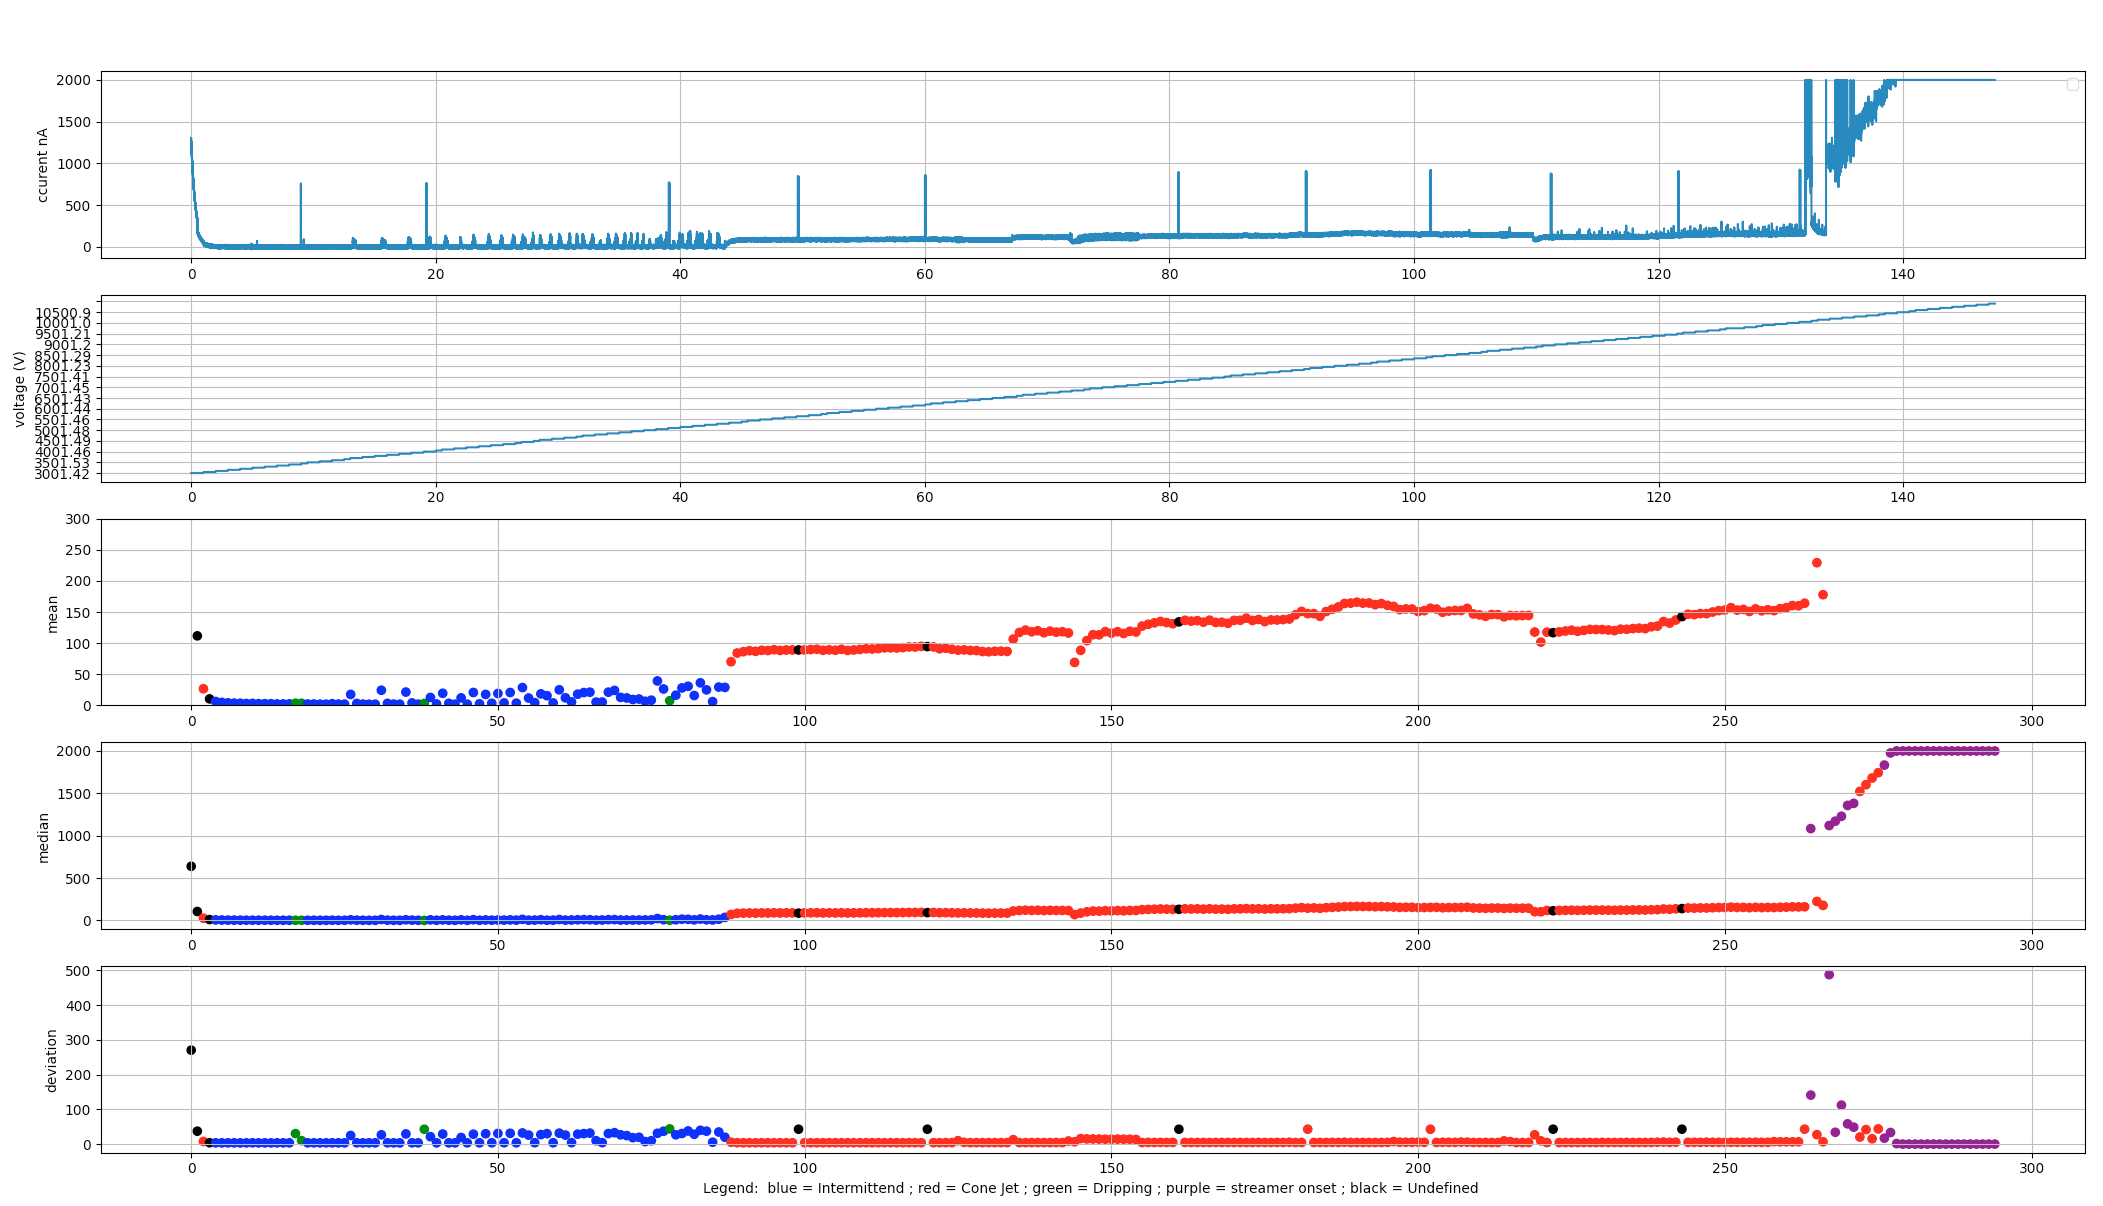
\includegraphics[width=17cm]{images/images_folder_3/data4.png}
%         \caption{Data acquired in the experiment 3 - pure ethanol}
%     \end{figure}

%     \begin{multicols}{3}

%         \begin{figure}[H]
%             \center
%             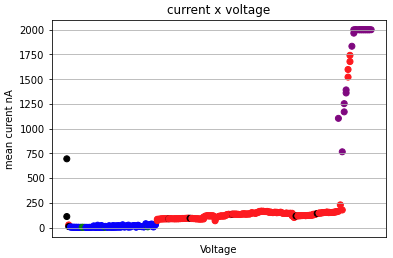
\includegraphics[width=5cm]{images/images_folder_3/data4_sjaakgraph1.png}
%             \caption{current mean X voltage}
%         \end{figure}

%         \begin{figure}[H]
%             \center
%             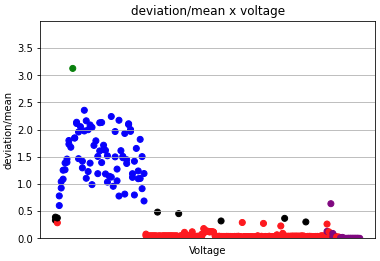
\includegraphics[width=5cm]{images/images_folder_3/data4_sjaakgraph2.png}
%             \caption{deviation/mean}
%         \end{figure}

%         \begin{figure}[H]
%             \center
%             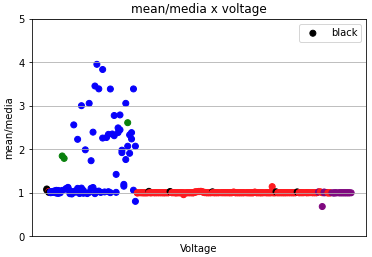
\includegraphics[width=5cm]{images/images_folder_3/data4_sjaakgraph3.png}
%             \caption{mean/median}
%         \end{figure}

%     \end{multicols}





